\documentclass[11pt]{scrartcl}
\usepackage{mm_ws15}
\usetikzlibrary{patterns}

\newcommand{\sheetTitle}{Blatt 0}
\begin{document}
\maketitle

\section*{Hinweise zum Übungsbetrieb}
\begin{itemize}
  \item Homepage zur Übung: \url{http://thp.uni-koeln.de/~dsuess/ws15/}
  \item Die \emph{Übungsaufgaben} werden immer Dienstag in der Vorlesung ausgegeben und auf oben genannter Seite zum Download zur Verfügung gestellt. Die \emph{Abgabe der Lösung} erfolgt eine Woche später \emph{bis spätestens Montag 12:00} in die Briefkästen vor dem Institut für Theoretische Physik (im Altbau).
  \item Heften Sie alle Blätter in der richtigen Reihenfolge zusammen und schreiben Sie Ihren Namen, die Nummer Ihrer Übungsgruppe und den Namen des Übungsgruppenleiters bzw. der Übungsgruppenleiterin auf die erste Seite. 
  \item Jede Teilnehmerin und jeder Teilnehmer dieser Vorlesung gibt eine eigene Version der Lösung ab. Wir ermuntern Sie ausdrücklich dazu, die Aufgaben in kleineren Gruppen zu bearbeiten und über möglichen Lösungswege zu diskutieren. Durch Abschreiben der Lösung von Ihren Kommilitonen und Kommilitoninnen geht Ihnen ein wichtiger Teil der Vorlesung verloren.
  \item Wenn Sie Schwierigkeiten mit dem Stoff haben und etwas nicht verstehen, versuchen Sie, diese Probleme umgehend zu beheben. Teile der Vorlesung bauen meist auf Vorangegangenes auf und Wissenslücken werden im Laufe des Semester immer schwieriger zu füllen sein. Anlaufstellen bei Fragen (in der Reihenfolge, wie sie auch aufgesucht werden sollten): Literatur, Ihre Kommilitonen/Kommilitoninnen, die Fragestunde (Freitag 12:00 HS2), die Übungen, der Lesende nach der Vorlesung.
  \item Zusätzlich haben wir für Sie einen Diskussionsbereich online eingerichtet, wo Sie mögliche Fragen jeder Zeit stellen (und auch beantworten) können. Diesen erreichen Sie unter \url{http://mathematische-methoden-ws15.wikispaces.com/}
\end{itemize}


\section*{Vorwissen}
Sie sollten mit den folgenden mathematischen Begriffen und Techniken aus der Schule vertraut sein. Falls nicht, sollten Sie dieses Defizit umgehend beheben.
\begin{itemize}
  \item Bruchrechnung
  \item Umstellung von Gleichung, Lösung von linearen Gleichungssystemen
  \item trigonometrischen Funktionen (z.B. Definition, Additionstheoreme, \ldots)
  \item Rechenregeln für Potenzfunktionen und Logarithmusfunktionen
  \item Differentialrechnung (Bedeutung und Definition der Ableitung, Ableitung elementarer Funktionen, Ableitungsregeln)
  \item Integralrechnung (bestimmte/unbestimmte Integration, Integrale elementarer Funktionen)
\end{itemize}
\vspace{1em}

Die folgende Aufgabe soll als Vorbereitung für die erste Übung am 22.10. dienen.
Wiederholen Sie die folgenden Begriffe mithilfe des 0.\ Kapitels der Vorlesung und der angegebenen Literatur (siehe Homepage der Vorlesung).
Beschäftigen Sie sich außerdem mit den unter \quotes{Vorwissen} angeführten Begriffen.

\section*{Aufgaben zur Vorbereitung}
Geben Sie zu jedem Begriff eine kurze Definition in eigenen Worten.
Wenn möglich, untermalen Sie die Aussagen mit geeigneten Beispielen.

\begin{description}[leftmargin=1cm,labelindent=1cm]
  \item[Mengen] Wie sind Teilmenge, Vereinigungsmenge, Schnittmenge und Produktmenge definiert?
  Was ist ein Venn-Diagramm?
  \item[Abbildungen] Definieren Sie die Begriffe injektive, bijektive und surjektive Abbildung. 
  Wann sind zwei Mengen gleichmächtig?
  \item[Vektorraum] Beschreiben sie kurz den Begriff des Vektorraumes. 
  Welche physikalische Größen werden durch Vektoren beschrieben und warum?
  \item[Lineare Unabhängigkeit] Was versteht man unter linearer Unabhängigkeit einer Menge von Vektoren? 
  Wann spricht man von einem Erzeugendensystem, wann von einer Basis? 
  \item[Stetigkeit und Differenzierbarkeit] Wann ist eine Funktion stetig, wann differenzierbar? 
  Impliziert Differenzierbarkeit auch Stetigkeit? 
  Geben Sie ein Beispiel und ein Gegenbeispiel an.
\end{description}

\sepline[.75\textwidth]

Der Rest dieses Blattes enthält eine Beispielübung mit Musterlösung und soll die Herangehensweise an typische Aufgaben illustrieren und beispielhaft zeigen, wie eine mögliche Darstellung der Lösung aussehen kann. 

\section{Elementare Rechenoperationen mit Vektoren}
\begin{subex}
  \item Berechnen Sie $\mat{a} + \mat{b}$, $\mat{a} - \mat{b}$, $5 \mat{a}$ und $3 \mat{a} + (-2) \mat{b}$ für $\mat{a} = \colvec{3 \\ 1}$ und $\mat{b} = \colvec{ -1 \\ 2 }$.
  \item Drücken Sie $\mat{a} = \colvec{ 1 \\ 3 }$ als Linearkombination von $\mat{e}_1 = \colvec{ 2 \\ 1 }$ und $\mat{e}_2 = \colvec{ 1 \\ -1 }$ aus.
\end{subex}

\begin{solution}
  \begin{subex}
  \item Addition und Subtraktion von Vektoren werden komponentenweise ausgeführt
  \[
    \mat{a} + \mat{b} = \colvec{ 3 \\ 1 } + \colvec{ -1 \\ 2 } = \colvec{ 3 + (-1) \\ 1 + 2 } = \colvec{ 2 \\ 3 }
  \]
  \[
    \mat{a} - \mat{b} = \colvec{ 3 \\ 1 } - \colvec{ -1 \\ 2 } = \colvec{ 3 - (-1) \\ 1 - 2 } = \colvec{ 4 \\ -1 }
  \]
  Multiplikation von Vektoren mit reellen Zahlen ebenso
  \[
    5 \mat{a} = 5 \colvec{ 3 \\ 1 } = \colvec{ 5 \times 3 \\ 5 \times 1 } = \colvec{ 15 \\ 5 }
  \]
  Nacheinanderausführung von Multiplikation und Addition (\quotes{Punkt- vor Strichrechnung}), ebenfalls komponentenweise
  \[
    3 \mat{a} + (-2) \mat{b} = \colvec{ 3 \times 3 \\ 3 \times 1 } + \colvec{ -2 \times (-1) \\ -2 \times 2 }
    = \colvec{ 9 \\ 3 } + \colvec{ 2 \\ -4 } = \colvec{ 11 \\ -1 }
  \]

  \item Stelle $\mat{a}$ als Linearkombination $x\times \mat{e}_1 + y\times \mat{e}_2$ dar, wobei die Koeffizienten $x,y \in \RR$ zunächst unbestimmt sind
  \[
    \mat{a} \stackrel{!}{=} x \times \mat{e}_1 + y \times \mat{e}_2
  \]
  Einsetzen liefert zwei Gleichungen für die Komponenten und somit ein lineares Gleichungssystem, das wir wie gewohnt lösen
  \begin{align*}
    \left\{ \begin{array}{l}1 = 2x + y \\  3 = x - y \end{array} \right. \quad [\,\,\rightarrow \mathrm{I + II}] \quad \left\{ \begin{array}{l}1 = 2x + y  \\  4 = 3x \end{array} \right.
  \end{align*}
  Ablesen und Rückeinsetzen liefert $x = \frac{4}{3}$, $y = 1 - 2x = -\frac{5}{3}$, also gilt $\mat{a} = \frac{4}{3}\times\mat{e}_1 - \frac{5}{3}\times \mat{e}_2$.
  \end{subex}
\end{solution}


\section{Abzählbarkeit von Mengen}
Häufig hat man es in der Mathematik mit unendlichen Mengen zu tun.
Um dennoch die Größe von zwei Mengen vergleichen zu können, wurde in der Vorlesung der Begriff der \emph{Gleichmächtigkeit} eingeführt.

Eine wichtige Familie von Mengen sind die \emph{abzählbaren Mengen}:
Eine Menge heißt abzählbar, wenn sie gleichmächtig zu einer Teilmenge von $\NN$ ist (d.h.\ gleichmächtig zu $\NN$ oder zu einer echten Teilmenge von $\NN$).
Beweisen Sie, dass die folgenden Mengen abzählbar sind.
  \begin{subex}
    \item $A = \{ \mathrm{Schere},\, \mathrm{Stein},\, \mathrm{Papier} \}$
    \item $G = \{ n \in \NN \vert n \mbox{ gerade} \}$
  \end{subex}  
\begin{solution}
  Diese Übungsaufgabe soll dazu dienen, die Technik des \emph{direkten Beweises} zu üben.
  \begin{subex}
    \item $A$ ist abzählbar, da $A$ eine endliche Menge ist. 
    Explizit lautet eine bijektive Abbildung $f\colon \NN_3 \rightarrow A$, die zwischen $\NN_3 = \{1, 2, 3\} \subset \NN$ und $A$ vermittelt
    \[
      f(1) = \mathrm{Schere}, \quad f(2) = \mathrm{Stein}, \quad f(3) = \mathrm{Papier}.
    \]
  $f$ ist injektiv, da jedem Element aus $\NN_3$ genau ein Element aus $A$ zugeordnet wird.
  $f$ ist surjektiv, da es für jedes Element aus $x \in A$ ein Element aus $n \in \NN_3$ gibt, sodass $f(n) = x$.

  \item Klar ist, dass $G$ eine unendliche Menge ist. 
  Eine Mögliche Abzählung $f$ lautet
  \[
    f\colon \NN \rightarrow G, n \mapsto f(n) = 2n.
  \]
  Natürlich hat jede gerade Zahl eine solche Darstellung.
  Mit anderen Worten: $f$ ist surjektiv.
  Andererseits wird jedem $n \in \NN$ genau ein Element aus $G$ zugeordnet, also ist $f$ injektiv.
  Dies sieht man noch deutlicher an folgendem Bild:

  \begin{center}
    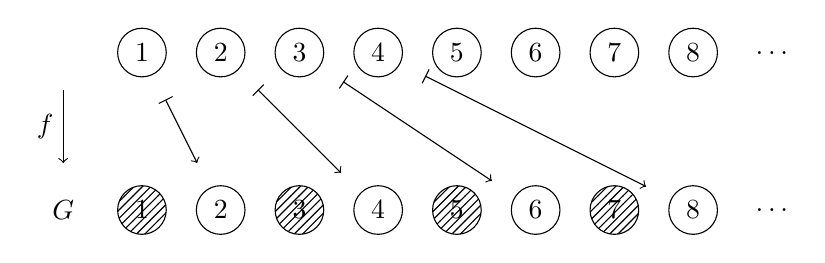
\begin{tikzpicture}[%
      element/.style={circle,draw,fill=white,minimum size=10},
      noelement/.style={circle,draw,pattern=north east lines,minimum size=10}
    ]
      \node (N) at (0, 2) {$\NN$};
      \node (G) at (0, 0) {$G$};
      \draw[->,shorten >= 10pt, shorten <= 10pt] (N) -- node[left] {$f$} ++ (G);

      \foreach \n in {1,...,4}{%
        \pgfmathtruncatemacro{\label}{2*\n - 1}
        \node [noelement]  (u\label) at (2*\n - 1,0) {\label};
        \node [element]  (o\label) at (2*\n - 1,2) {\label};
      } 
      \foreach \n in {1,...,4}{%
        \pgfmathtruncatemacro{\label}{2*\n}
        \node [element]  (u\label) at (2*\n,0) {\label};
        \node [element]  (o\label) at (2*\n,2) {\label};

      \draw[|->,shorten >= 10pt, shorten <= 10pt] (o\n) -- (u\label);

      } 

      \node at (9, 2) {$\ldots$};
      \node at (9, 0) {$\ldots$};

    \end{tikzpicture}
  \end{center}

  Das heißt, dass obwohl $G$ eine echte Teilmenge von $\NN$ ist, sind beide dennoch gleichmächtig --  eine Besonderheit von unendlichen Mengen.
  \end{subex}
\end{solution}

\end{document}
